\documentclass{standalone}
\usepackage{tikz}
\usetikzlibrary{patterns, positioning}
\usetikzlibrary{shapes.misc}
\usepackage[outline]{contour}
\contourlength{1.5pt} 
\usepackage[sfdefault]{ClearSans} %% option 'sfdefault' activates Clear Sans as the default text font
\usepackage[T1]{fontenc}

\begin{document}
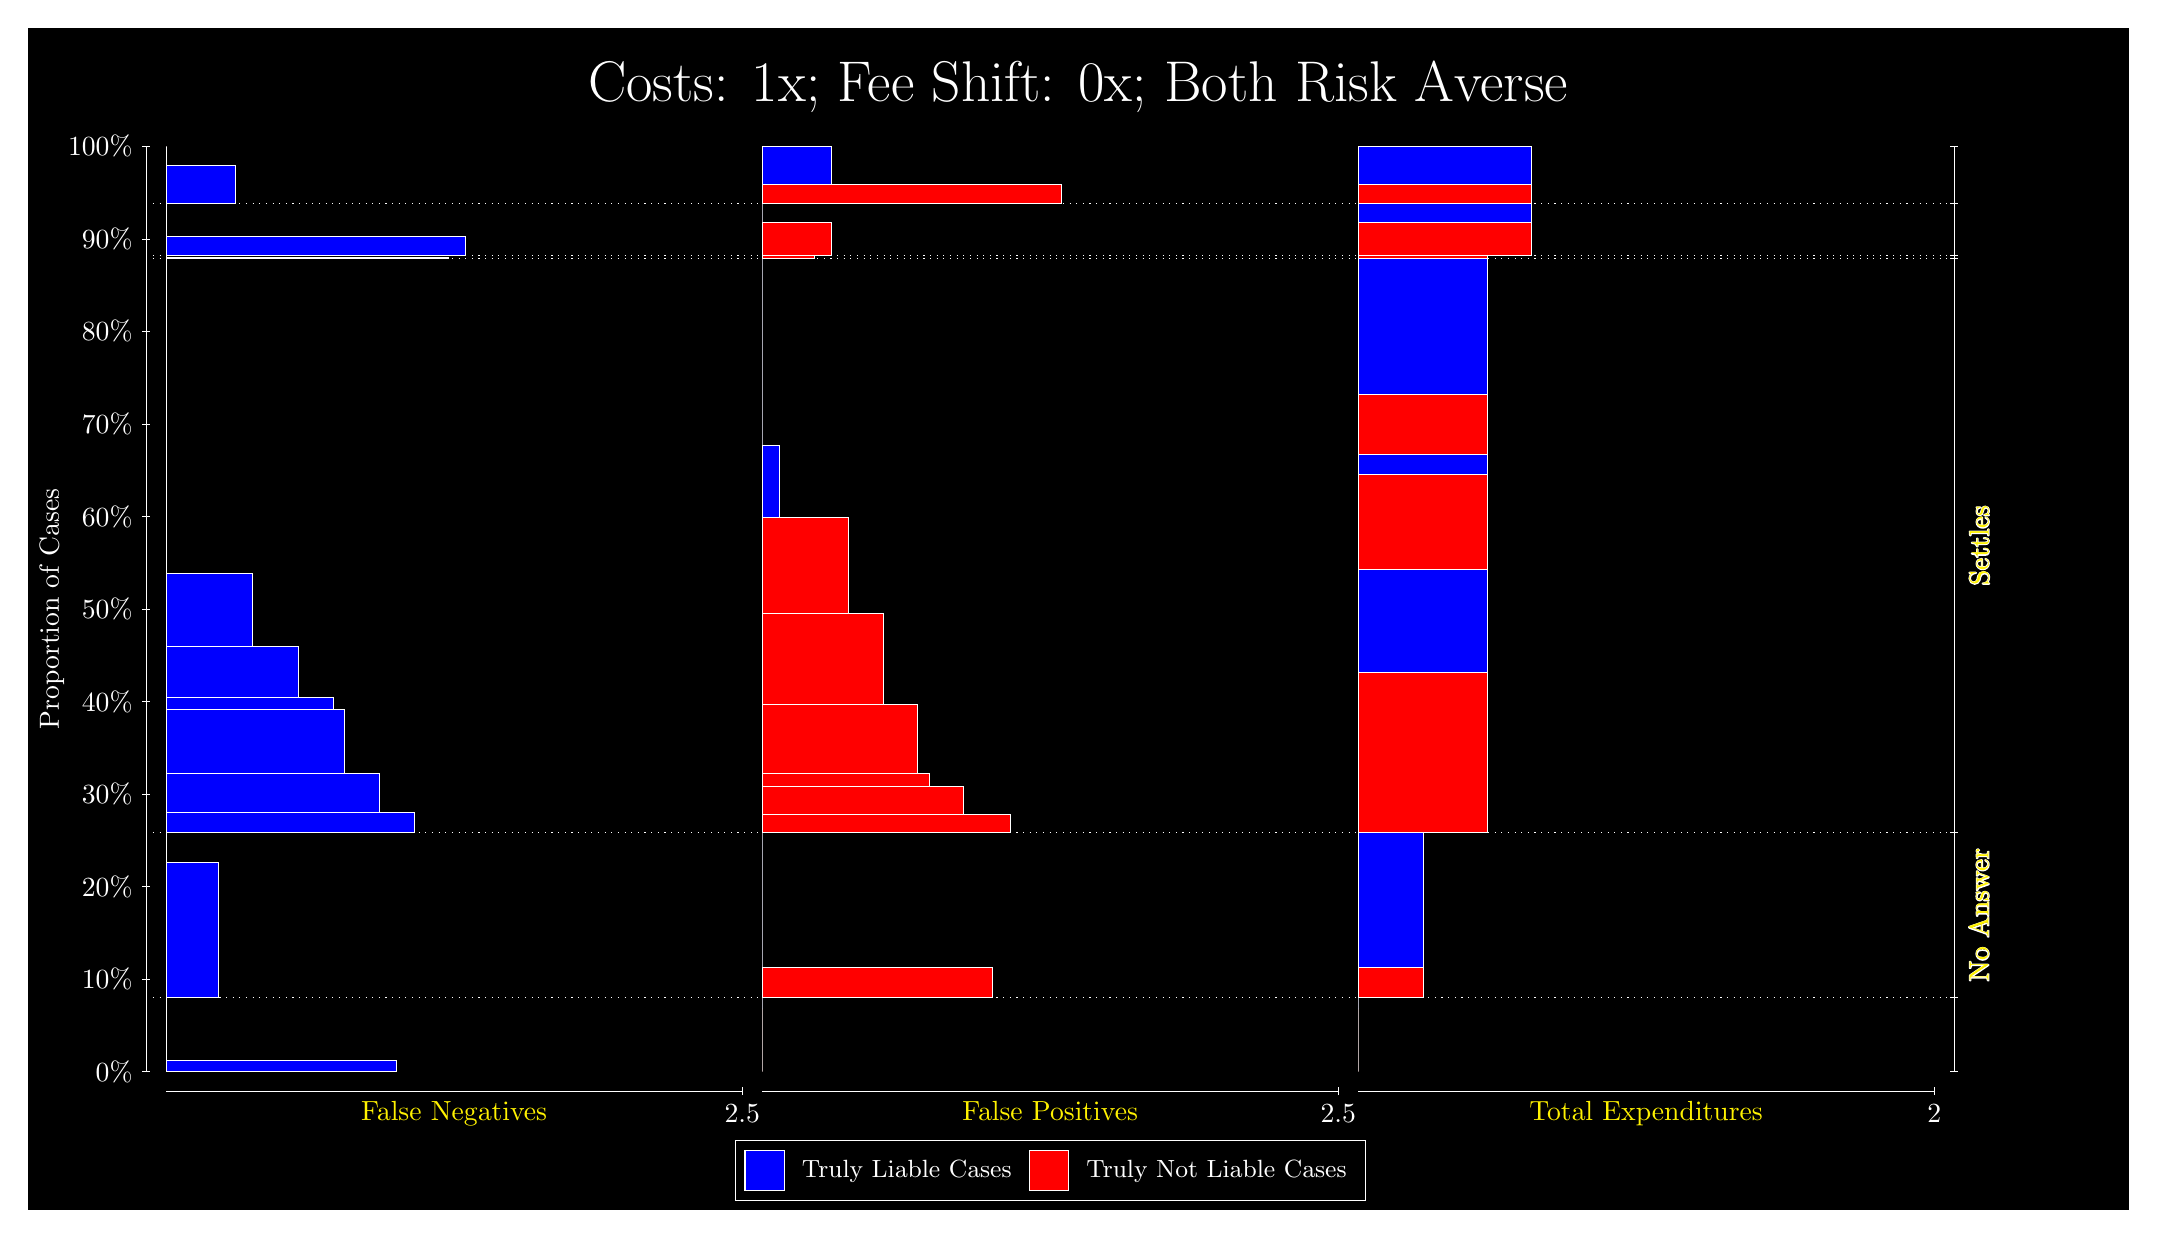
\begin{tikzpicture}
\draw[fill=black] (0,0) rectangle (26.667,15);
\draw[text=white] (0,13.5) rectangle (26.667,15) node[midway] {\huge Costs: 1x; Fee Shift: 0x; Both Risk Averse};
\draw[white, very thin] (1.5,1.75) -- (1.5,13.5);
\node[rotate=90, text=white, anchor=center] at (0.3, 7.625) {Proportion of Cases};
\draw[white, very thin] (1.45,1.75) -- (1.55,1.75);
\node[text=white, anchor=east] at (1.45, 1.75) {0\%};
\draw[white, very thin] (1.45,2.925) -- (1.55,2.925);
\node[text=white, anchor=east] at (1.45, 2.925) {10\%};
\draw[white, very thin] (1.45,4.1) -- (1.55,4.1);
\node[text=white, anchor=east] at (1.45, 4.1) {20\%};
\draw[white, very thin] (1.45,5.275) -- (1.55,5.275);
\node[text=white, anchor=east] at (1.45, 5.275) {30\%};
\draw[white, very thin] (1.45,6.45) -- (1.55,6.45);
\node[text=white, anchor=east] at (1.45, 6.45) {40\%};
\draw[white, very thin] (1.45,7.625) -- (1.55,7.625);
\node[text=white, anchor=east] at (1.45, 7.625) {50\%};
\draw[white, very thin] (1.45,8.8) -- (1.55,8.8);
\node[text=white, anchor=east] at (1.45, 8.8) {60\%};
\draw[white, very thin] (1.45,9.975) -- (1.55,9.975);
\node[text=white, anchor=east] at (1.45, 9.975) {70\%};
\draw[white, very thin] (1.45,11.15) -- (1.55,11.15);
\node[text=white, anchor=east] at (1.45, 11.15) {80\%};
\draw[white, very thin] (1.45,12.325) -- (1.55,12.325);
\node[text=white, anchor=east] at (1.45, 12.325) {90\%};
\draw[white, very thin] (1.45,13.5) -- (1.55,13.5);
\node[text=white, anchor=east] at (1.45, 13.5) {100\%};

\draw[white, very thin] (24.457,1.75) -- (24.457,13.5);
\draw[white, very thin] (24.407,1.75) -- (24.507,1.75);
\node[anchor=west] at (24.407, 1.75) {};
\draw[white, very thin] (24.407,2.6953) -- (24.507,2.6953);
\node[anchor=west] at (24.407, 2.6953) {};
\draw[white, very thin] (24.407,4.7833) -- (24.507,4.7833);
\node[anchor=west] at (24.407, 4.7833) {};
\draw[white, very thin] (24.407,12.077) -- (24.507,12.077);
\node[anchor=west] at (24.407, 12.077) {};
\draw[white, very thin] (24.407,12.119) -- (24.507,12.119);
\node[anchor=west] at (24.407, 12.119) {};
\draw[white, very thin] (24.407,12.775) -- (24.507,12.775);
\node[anchor=west] at (24.407, 12.775) {};
\draw[white, very thin] (24.407,13.5) -- (24.507,13.5);
\node[anchor=west] at (24.407, 13.5) {};

\draw[white, very thin, fill=blue] (1.75,1.75) rectangle (4.6775,1.8987);
\draw[white, very thin, fill=red] (1.75,1.8987) rectangle (1.75,2.6953);
\draw[white, very thin, fill=blue] (1.75,2.6953) rectangle (2.4087,4.4034);
\draw[white, very thin, fill=red] (1.75,4.4034) rectangle (1.75,4.7833);
\draw[white, very thin, fill=blue] (1.75,4.7833) rectangle (4.8971,5.0403);
\draw[white, very thin, fill=blue] (1.75,5.0403) rectangle (4.458,5.5359);
\draw[white, very thin, fill=blue] (1.75,5.5359) rectangle (4.0188,6.3492);
\draw[white, very thin, fill=blue] (1.75,6.3492) rectangle (3.8725,6.5045);
\draw[white, very thin, fill=blue] (1.75,6.5045) rectangle (3.4333,7.1544);
\draw[white, very thin, fill=blue] (1.75,7.1544) rectangle (2.8478,8.0777);
\draw[white, very thin, fill=red] (1.75,8.0777) rectangle (1.75,12.077);
\draw[white, very thin, fill=blue] (1.75,12.077) rectangle (5.3362,12.086);
\draw[white, very thin, fill=red] (1.75,12.086) rectangle (1.75,12.119);
\draw[white, very thin, fill=blue] (1.75,12.119) rectangle (5.5558,12.354);
\draw[white, very thin, fill=red] (1.75,12.354) rectangle (1.75,12.775);
\draw[white, very thin, fill=blue] (1.75,12.775) rectangle (2.6283,13.253);
\draw[white, very thin, fill=red] (1.75,13.253) rectangle (1.75,13.5);
\draw[white, very thin, fill=red] (9.3189,1.75) rectangle (9.3189,2.5466);
\draw[white, very thin, fill=blue] (9.3189,2.5466) rectangle (9.3189,2.6953);
\draw[white, very thin, fill=red] (9.3189,2.6953) rectangle (12.246,3.0752);
\draw[white, very thin, fill=blue] (9.3189,3.0752) rectangle (9.3189,4.7833);
\draw[white, very thin, fill=red] (9.3189,4.7833) rectangle (12.466,5.0232);
\draw[white, very thin, fill=red] (9.3189,5.0232) rectangle (11.88,5.3731);
\draw[white, very thin, fill=red] (9.3189,5.3731) rectangle (11.441,5.5412);
\draw[white, very thin, fill=red] (9.3189,5.5412) rectangle (11.295,6.4203);
\draw[white, very thin, fill=red] (9.3189,6.4203) rectangle (10.856,7.5745);
\draw[white, very thin, fill=red] (9.3189,7.5745) rectangle (10.417,8.783);
\draw[white, very thin, fill=blue] (9.3189,8.783) rectangle (9.5384,9.7063);
\draw[white, very thin, fill=blue] (9.3189,9.7063) rectangle (9.3189,12.077);
\draw[white, very thin, fill=red] (9.3189,12.077) rectangle (9.9776,12.11);
\draw[white, very thin, fill=blue] (9.3189,12.11) rectangle (9.3189,12.119);
\draw[white, very thin, fill=red] (9.3189,12.119) rectangle (10.197,12.539);
\draw[white, very thin, fill=blue] (9.3189,12.539) rectangle (9.3189,12.775);
\draw[white, very thin, fill=red] (9.3189,12.775) rectangle (13.125,13.021);
\draw[white, very thin, fill=blue] (9.3189,13.021) rectangle (10.197,13.5);
\draw[white, very thin, fill=red] (16.888,1.75) rectangle (16.888,2.5466);
\draw[white, very thin, fill=blue] (16.888,2.5466) rectangle (16.888,2.6953);
\draw[white, very thin, fill=red] (16.888,2.6953) rectangle (17.711,3.0752);
\draw[white, very thin, fill=blue] (16.888,3.0752) rectangle (17.711,4.7833);
\draw[white, very thin, fill=red] (16.888,4.7833) rectangle (18.534,6.8166);
\draw[white, very thin, fill=blue] (16.888,6.8166) rectangle (18.534,8.1255);
\draw[white, very thin, fill=red] (16.888,8.1255) rectangle (18.534,9.334);
\draw[white, very thin, fill=blue] (16.888,9.334) rectangle (18.534,9.591);
\draw[white, very thin, fill=red] (16.888,9.591) rectangle (18.534,10.349);
\draw[white, very thin, fill=blue] (16.888,10.349) rectangle (18.534,12.077);
\draw[white, very thin, fill=red] (16.888,12.077) rectangle (18.534,12.11);
\draw[white, very thin, fill=blue] (16.888,12.11) rectangle (18.534,12.119);
\draw[white, very thin, fill=red] (16.888,12.119) rectangle (19.083,12.539);
\draw[white, very thin, fill=blue] (16.888,12.539) rectangle (19.083,12.775);
\draw[white, very thin, fill=red] (16.888,12.775) rectangle (19.083,13.021);
\draw[white, very thin, fill=blue] (16.888,13.021) rectangle (19.083,13.5);
\draw[white, dotted] (1.5,2.6953) -- (24.457,2.6953);
\draw[white, dotted] (1.5,4.7833) -- (24.457,4.7833);
\draw[white, dotted] (1.5,12.077) -- (24.457,12.077);
\draw[white, dotted] (1.5,12.119) -- (24.457,12.119);
\draw[white, dotted] (1.5,12.775) -- (24.457,12.775);
\draw[white, very thin] (1.75,1.5) -- (9.0689,1.5);
\node[text=yellow, anchor=north] at (5.4094, 1.5) {False Negatives};
\draw[white, very thin] (9.0689,1.45) -- (9.0689,1.55);
\node[text=white, anchor=north] at (9.0689, 1.45) {2.5};

\draw[white, very thin] (9.3189,1.5) -- (16.638,1.5);
\node[text=yellow, anchor=north] at (12.978, 1.5) {False Positives};
\draw[white, very thin] (16.638,1.45) -- (16.638,1.55);
\node[text=white, anchor=north] at (16.638, 1.45) {2.5};

\draw[white, very thin] (16.888,1.5) -- (24.207,1.5);
\node[text=yellow, anchor=north] at (20.547, 1.5) {Total Expenditures};
\draw[white, very thin] (24.207,1.45) -- (24.207,1.55);
\node[text=white, anchor=north] at (24.207, 1.45) {2};


\node[text=yellow, centered, rotate=90] at (24.777, 3.7393) {\contour{white}{No Answer}};
\node[text=yellow, centered, rotate=90] at (24.777, 8.4303) {\contour{white}{Settles}};




\draw (12.978300999999998,1.5) node[draw=none] (baseCoordinate) {};
\begin{scope}[align=center]
        \matrix[scale=0.5, draw=white, below=0.5cm of baseCoordinate, nodes={draw}, column sep=0.1cm]{
            \node[rectangle, draw, minimum width=0.5cm, minimum height=0.5cm, fill=blue] {}; &
            \node[draw=none, font=\small, text=white] (B) {Truly Liable Cases}; &
            \node[rectangle, draw, minimum width=0.5cm, minimum height=0.5cm, fill=red] {}; &
            \node[draw=none, font=\small, text=white] (B) {Truly Not Liable Cases}; \\
            };
\end{scope}

\end{tikzpicture}
\end{document}